% -*- root: ../main.tex -*-

% Riassumere le soluzioni presenti in letteratura inerenti al problema in esame. Per ciascuna, discutere le principali diversità o affinità rispetto al progetto presentato. Nel caso non siano presenti soluzioni direttamente comparabili a quella presentata descrivere comunque le principali tecniche note per affrontare la tematica trattata. Le soluzioni esposte devono essere corredate degli opportuni riferimenti bibliografici. Nel caso si tratti di soluzioni già operative sul mercato, devono essere indicate le fonti (online) dove poter accedere al servizio o approfondirne i contenuti.
% 3000 - 6000 battute

\chapter{Stato dell'Arte}
Il topic scelto non gode di particolare attenzione in letteratura.
Dalle informazioni che abbiamo raccolto su ricerche, studi e applicazione di \textbf{idee similari} alla nostra è emerso quanto segue:

\begin{itemize}
    \item \textbf{Automazione}: sono state condotte alcune ricerche che riguardano interventi di \textbf{automazione} del sistema di alimentazione per gli allevamenti, ma si tratta di progetti con un forte imprinting \textbf{economico}. 
    \item \textbf{Distribuzione del cibo}: alcune soluzioni commerciali offrono la \textbf{distribuzione automatica }del cibo ad orari \textbf{temporizzati}, senza possibilità di \textbf{dosaggio} o di rilevamento dei \textbf{consumi}.
    \item \textbf{Monitoraggio parametri}: in ambito commerciale esistono soluzioni che si focalizzano soprattutto sul \textbf{monitoraggio} e la \textbf{notifica} dei \textbf{parametri vitali} dell'animale.
    \item \textbf{Fusione dei due ambiti}: \textbf{non} siamo riusciti a trovare progetti che fondono i due ambiti come invece fa la nostra proposta. La \textbf{nostra} soluzione, infatti, tenta di \textbf{fondere} le due idee e di proporre un \textbf{sistema remoto} e \textbf{scalabile}, che monitori i \textbf{parametri vitali}, che possa anche fornire un automatismo alla gestione del \textbf{cibo} e dell'\textbf{acqua} erogati al cane e, inoltre, che sia in grado sia di \textbf{intercettare} la presenza di \textbf{sintomi} riguardanti il consumo di cibo e acqua in base all'\textbf{analisi} dei dati raccolti.
\end{itemize}
 



Per quanto riguarda, invece, l'ambito dei \textbf{sensori}; lo stato dell'arte è in continua evoluzione, e possiamo trovare:
\begin{itemize}
    \item \textbf{\href{https://ciigar.csc.ncsu.edu/files/bib/Brugarolas2015-DogHeartMonitor.pdf}{Sensori ad hoc}}: impiegati nell'ambito della \textbf{ricerca} per il monitoraggio dei parametri vitali dei cani
    \item \textbf{\href{https://petpace.com/}{Collari smart}}: che si basano su un'idea simile alla nostra ma sono sistemi \textbf{proprietari}, commercializzati come prodotti ad uso domestico, completi di gps e altri sensori e supportati da un'\textbf{applicazione} che si rifà a quelle per gli smartwatch. Il costo di questi collari è dell'ordine delle centinaia di euro e deve essere associato ad un \textbf{abbonamento} mensile o annuale. 
    
    %PETPACE
    \begin{figure}[H]
       
        \label{fig:PetPace}
        \centering
        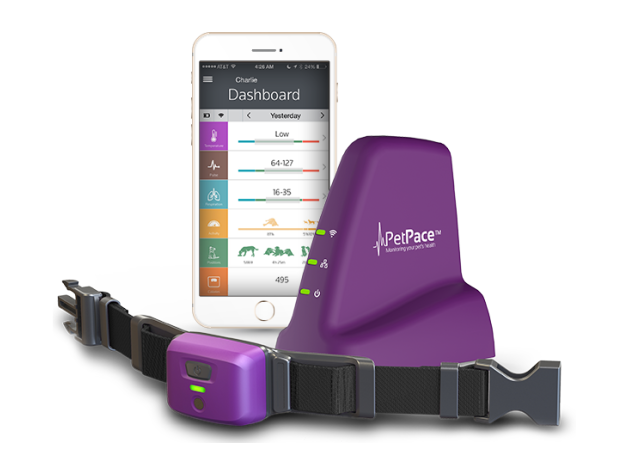
\includegraphics[width=0.8\textwidth]{Images/petpace.png}
         \caption{\textbf{Pet Pace}: uno dei collari smart in commercio basati su un'idea simile alla nostra}
    \end{figure}
\end{itemize}



I sensori di battiti tradizionali utilizzano un fascio luminoso per identificare la frequenza del battito cardiaco. Questa tecnologia si presta male per gli animali che presentano del pelo, come i cani, per questo sono in via di sviluppo sensori specifici che utilizzano principi diversi. Attualmente sono in corso delle
\href{https://vcs.vetmed.wsu.edu/research/clinical-studies/clinincal-studies-detail/vcs-clinical-studies/2017/06/28/new-ecg-technology}{ricerche} su sensori di altro genere che possano essere adatti anche anche ai cani.

\begin{tcolorbox}[width=12.1cm]
\begin{frame}{Lorem Ipsum}
    \begin{multicols}{2} % two columns
            I sensori di battiti tradizionali utilizzano un fascio luminoso per identificare la frequenza del battito cardiaco. Questa tecnologia si presta male per gli animali che presentano del pelo, come i cani, per questo sono in via di sviluppo sensori specifici che utilizzano principi diversi. Attualmente sono in corso delle
            \href{https://vcs.vetmed.wsu.edu/research/clinical-studies/clinincal-studies-detail/vcs-clinical-studies/2017/06/28/new-ecg-technology}{ricerche} su sensori di altro genere che possano essere adatti anche anche ai cani.
            Nonostante ciò la nostra soluzione utilizza un sensore
            \href{https://www.amazon.it/Haljia-Sensore-frequenza-cardiaca-Raspberry/dp/B01CBGH4N6}{classico}. Presupponendo che si utilizzi un collare smart solo per gli animali che, a causa del loro stato di salute, sono in osservazione, è possibile supporre che il pelo possa essere rasato durante il periodo di degenza.

    %CANILI
        \begin{figure}[H]
            \caption{I due canili interpellati in qualità di \textbf{esperti del dominio}}
            \label{fig:Canili}
            \centering
            
\includegraphics[width=0.3\textwidth]{Images/canili.png}
        \end{figure}
    \end{multicols}
\end{frame}
\end{tcolorbox}

Nonostante ciò la nostra soluzione utilizza un sensore
\href{https://www.amazon.it/Haljia-Sensore-frequenza-cardiaca-Raspberry/dp/B01CBGH4N6}{classico}. Presupponendo che si utilizzi un collare smart solo per gli animali che, a causa del loro stato di salute, sono in osservazione, è possibile supporre che il pelo possa essere rasato durante il periodo di degenza.

Per quanto riguarda le soluzioni riguardanti l'automatizzazione del cibo e dell'acqua le soluzioni commerciali sono davvero \href{https://www.fruugo.it/alimentatore-automatico-per-animali-domestici-a-43-l-capacita-alimentatore-intelligente-per-alimentazione-intelligente-per-lalimentazione-del-tempo-e-razionale-con-telecamera-telecomandato-tipo-di-lusso/p-55093501-111996468?language=it&ac=croud}{tante} molto simili.

Da questo punto di vista la nostra soluzione può dirsi all'avanguardia pur non essendo incentrata sull'uso domestico. Grossa parte di questi sistemi, infatti, usano: sensori del livello dell'acqua, bilance e sensori luminosi.
Inoltre alcuni sistemi più all'avanguardia consentono, tramite l'utilizzo di tecnologie come \textbf{BLE}, di monitorare da \textbf{App} i consumi e gli allarmi, non fornendo però alcun tipo di inferenza.

Attualmente il nostro sistema fornisce un'inferenza banale, ciò non toglie che in un futuro sviluppo associato ad uno studio comportamentale dell'animale non sia possibile implementare inferenze più complesse.

Quanto appena detto costituisce lo stato dell'arte nell'uso commerciale.
Per quanto riguarda lo specifico ambito del canile, invece, non sono state trovate applicazioni simili.

Per avere una visione più chiara di quello che è lo stato dei canili in Italia ci siamo rivolti a due \textbf{canili}:
\begin{itemize}
    \item \textbf{ACPA - Canile intercomunale di Cesena} Ci siamo recati fisicamente al canile di Cesena per discutere e toccare con mano lo stato tecnologico dello stabile, questo per valutare la fattibilità e la bontà della nostra soluzione.
    \item \textbf{Canile intercomunale "Soffio di Vento"- Pisa} Abbiamo contattato in via totalmente telematica il canile per comprendere se una soluzione del genere esistesse o fosse adottata da qualche parte e per avere una visione concreta dei problemi che vengono riscontrati per i quali avremmo potuto proporre una soluzione.
\end{itemize}

Entrambe le fonti ci hanno confermato che almeno in Italia lo stato dei canili risulta essere tecnologicamente obsoleto.
La soluzione proposta ha ricevuto un caloroso interesse da parte di entrambi i canili, con particolare entusiasmo per le rilevazioni dei consumi e il monitoraggio dei parametri vitali, con notifiche in caso di rilevazioni anomale.
Attualmente i canili contattati sono privi di una qualunque forma di \textbf{monitoraggio}, o \textbf{automatizzazione} di qualunque genere.
Il punto di forza di questo progetto risiede nella sua semplicità di dispiegamento, nelle tecnologie altamente accessibili e nel fatto che molti canili avrebbero il bisogno di una soluzione simile.
Il \textbf{collare} e l'\textbf{inferenza} sui consumi sono la parte che ha riscosso più successo poiché l'automatizzazione presenta alcuni svantaggi.
A detta del canile di Cesena dipende dalle norme del canile e dal modo con cui si vogliono addestrare i cani poiché buona parte delle pratiche di addestramento ruota attorno al cibo, che viene utilizzato sia come premio che come modo per far si che l'umano venga percepito come alpha.
La più grande critica mossa riguarda il fatto che se l'animale viene nutrito in maniera automatica allora non sarà abituato a ricevere cibo da persone, ed essendo l'adozione dei cani lo scopo principe del canile è probabile che il sistema automatizzato venga adottato solo da canili di grandezza medio-grande o la quale gestione non prevede l'addestramento. 